% Options for packages loaded elsewhere
\PassOptionsToPackage{unicode}{hyperref}
\PassOptionsToPackage{hyphens}{url}
%
\documentclass[
]{article}
\usepackage{amsmath,amssymb}
\usepackage{lmodern}
\usepackage{iftex}
\ifPDFTeX
  \usepackage[T1]{fontenc}
  \usepackage[utf8]{inputenc}
  \usepackage{textcomp} % provide euro and other symbols
\else % if luatex or xetex
  \usepackage{unicode-math}
  \defaultfontfeatures{Scale=MatchLowercase}
  \defaultfontfeatures[\rmfamily]{Ligatures=TeX,Scale=1}
\fi
% Use upquote if available, for straight quotes in verbatim environments
\IfFileExists{upquote.sty}{\usepackage{upquote}}{}
\IfFileExists{microtype.sty}{% use microtype if available
  \usepackage[]{microtype}
  \UseMicrotypeSet[protrusion]{basicmath} % disable protrusion for tt fonts
}{}
\makeatletter
\@ifundefined{KOMAClassName}{% if non-KOMA class
  \IfFileExists{parskip.sty}{%
    \usepackage{parskip}
  }{% else
    \setlength{\parindent}{0pt}
    \setlength{\parskip}{6pt plus 2pt minus 1pt}}
}{% if KOMA class
  \KOMAoptions{parskip=half}}
\makeatother
\usepackage{xcolor}
\usepackage[margin=1in]{geometry}
\usepackage{graphicx}
\makeatletter
\def\maxwidth{\ifdim\Gin@nat@width>\linewidth\linewidth\else\Gin@nat@width\fi}
\def\maxheight{\ifdim\Gin@nat@height>\textheight\textheight\else\Gin@nat@height\fi}
\makeatother
% Scale images if necessary, so that they will not overflow the page
% margins by default, and it is still possible to overwrite the defaults
% using explicit options in \includegraphics[width, height, ...]{}
\setkeys{Gin}{width=\maxwidth,height=\maxheight,keepaspectratio}
% Set default figure placement to htbp
\makeatletter
\def\fps@figure{htbp}
\makeatother
\setlength{\emergencystretch}{3em} % prevent overfull lines
\providecommand{\tightlist}{%
  \setlength{\itemsep}{0pt}\setlength{\parskip}{0pt}}
\setcounter{secnumdepth}{-\maxdimen} % remove section numbering
\ifLuaTeX
  \usepackage{selnolig}  % disable illegal ligatures
\fi
\IfFileExists{bookmark.sty}{\usepackage{bookmark}}{\usepackage{hyperref}}
\IfFileExists{xurl.sty}{\usepackage{xurl}}{} % add URL line breaks if available
\urlstyle{same} % disable monospaced font for URLs
\hypersetup{
  pdftitle={EDLD652 Presentation},
  pdfauthor={Sam Lorenzo},
  hidelinks,
  pdfcreator={LaTeX via pandoc}}

\title{EDLD652 Presentation}
\author{Sam Lorenzo}
\date{2023-03-11}

\begin{document}
\maketitle

\hypertarget{rethinking-traditional-values-analyzing-how-messages-of-climate-change-affect-family-planning-among-millennials-and-generation-z-phase-i---ghana}{%
\section{Rethinking Traditional Values: Analyzing How Messages of
Climate Change Affect Family Planning Among Millennials and Generation Z
(Phase I -
Ghana)}\label{rethinking-traditional-values-analyzing-how-messages-of-climate-change-affect-family-planning-among-millennials-and-generation-z-phase-i---ghana}}

\hypertarget{authors-samantha-lorenzo-laura-gattis}{%
\subsubsection{Authors: Samantha Lorenzo \& Laura
Gattis}\label{authors-samantha-lorenzo-laura-gattis}}

\begin{figure}
\centering
\includegraphics{https://png.pngtree.com/png-clipart/20221015/ourmid/pngtree-vintage-ghana-flag-png-image_6342465.png}
\caption{Ghana Flag}
\end{figure}

\begin{center}\rule{0.5\linewidth}{0.5pt}\end{center}

\hypertarget{warning}{%
\subsection{\texorpdfstring{\protect\includegraphics{https://static.vecteezy.com/system/resources/previews/009/663/747/original/warning-icon-transparent-free-png.png}}{Warning}}\label{warning}}

\begin{figure}
\centering
\includegraphics{https://pngimg.com/d/under_construction_PNG68.png}
\caption{Under Construction}
\end{figure}

\begin{center}\rule{0.5\linewidth}{0.5pt}\end{center}

\hypertarget{background}{%
\section{BACKGROUND}\label{background}}

\begin{figure}
\centering
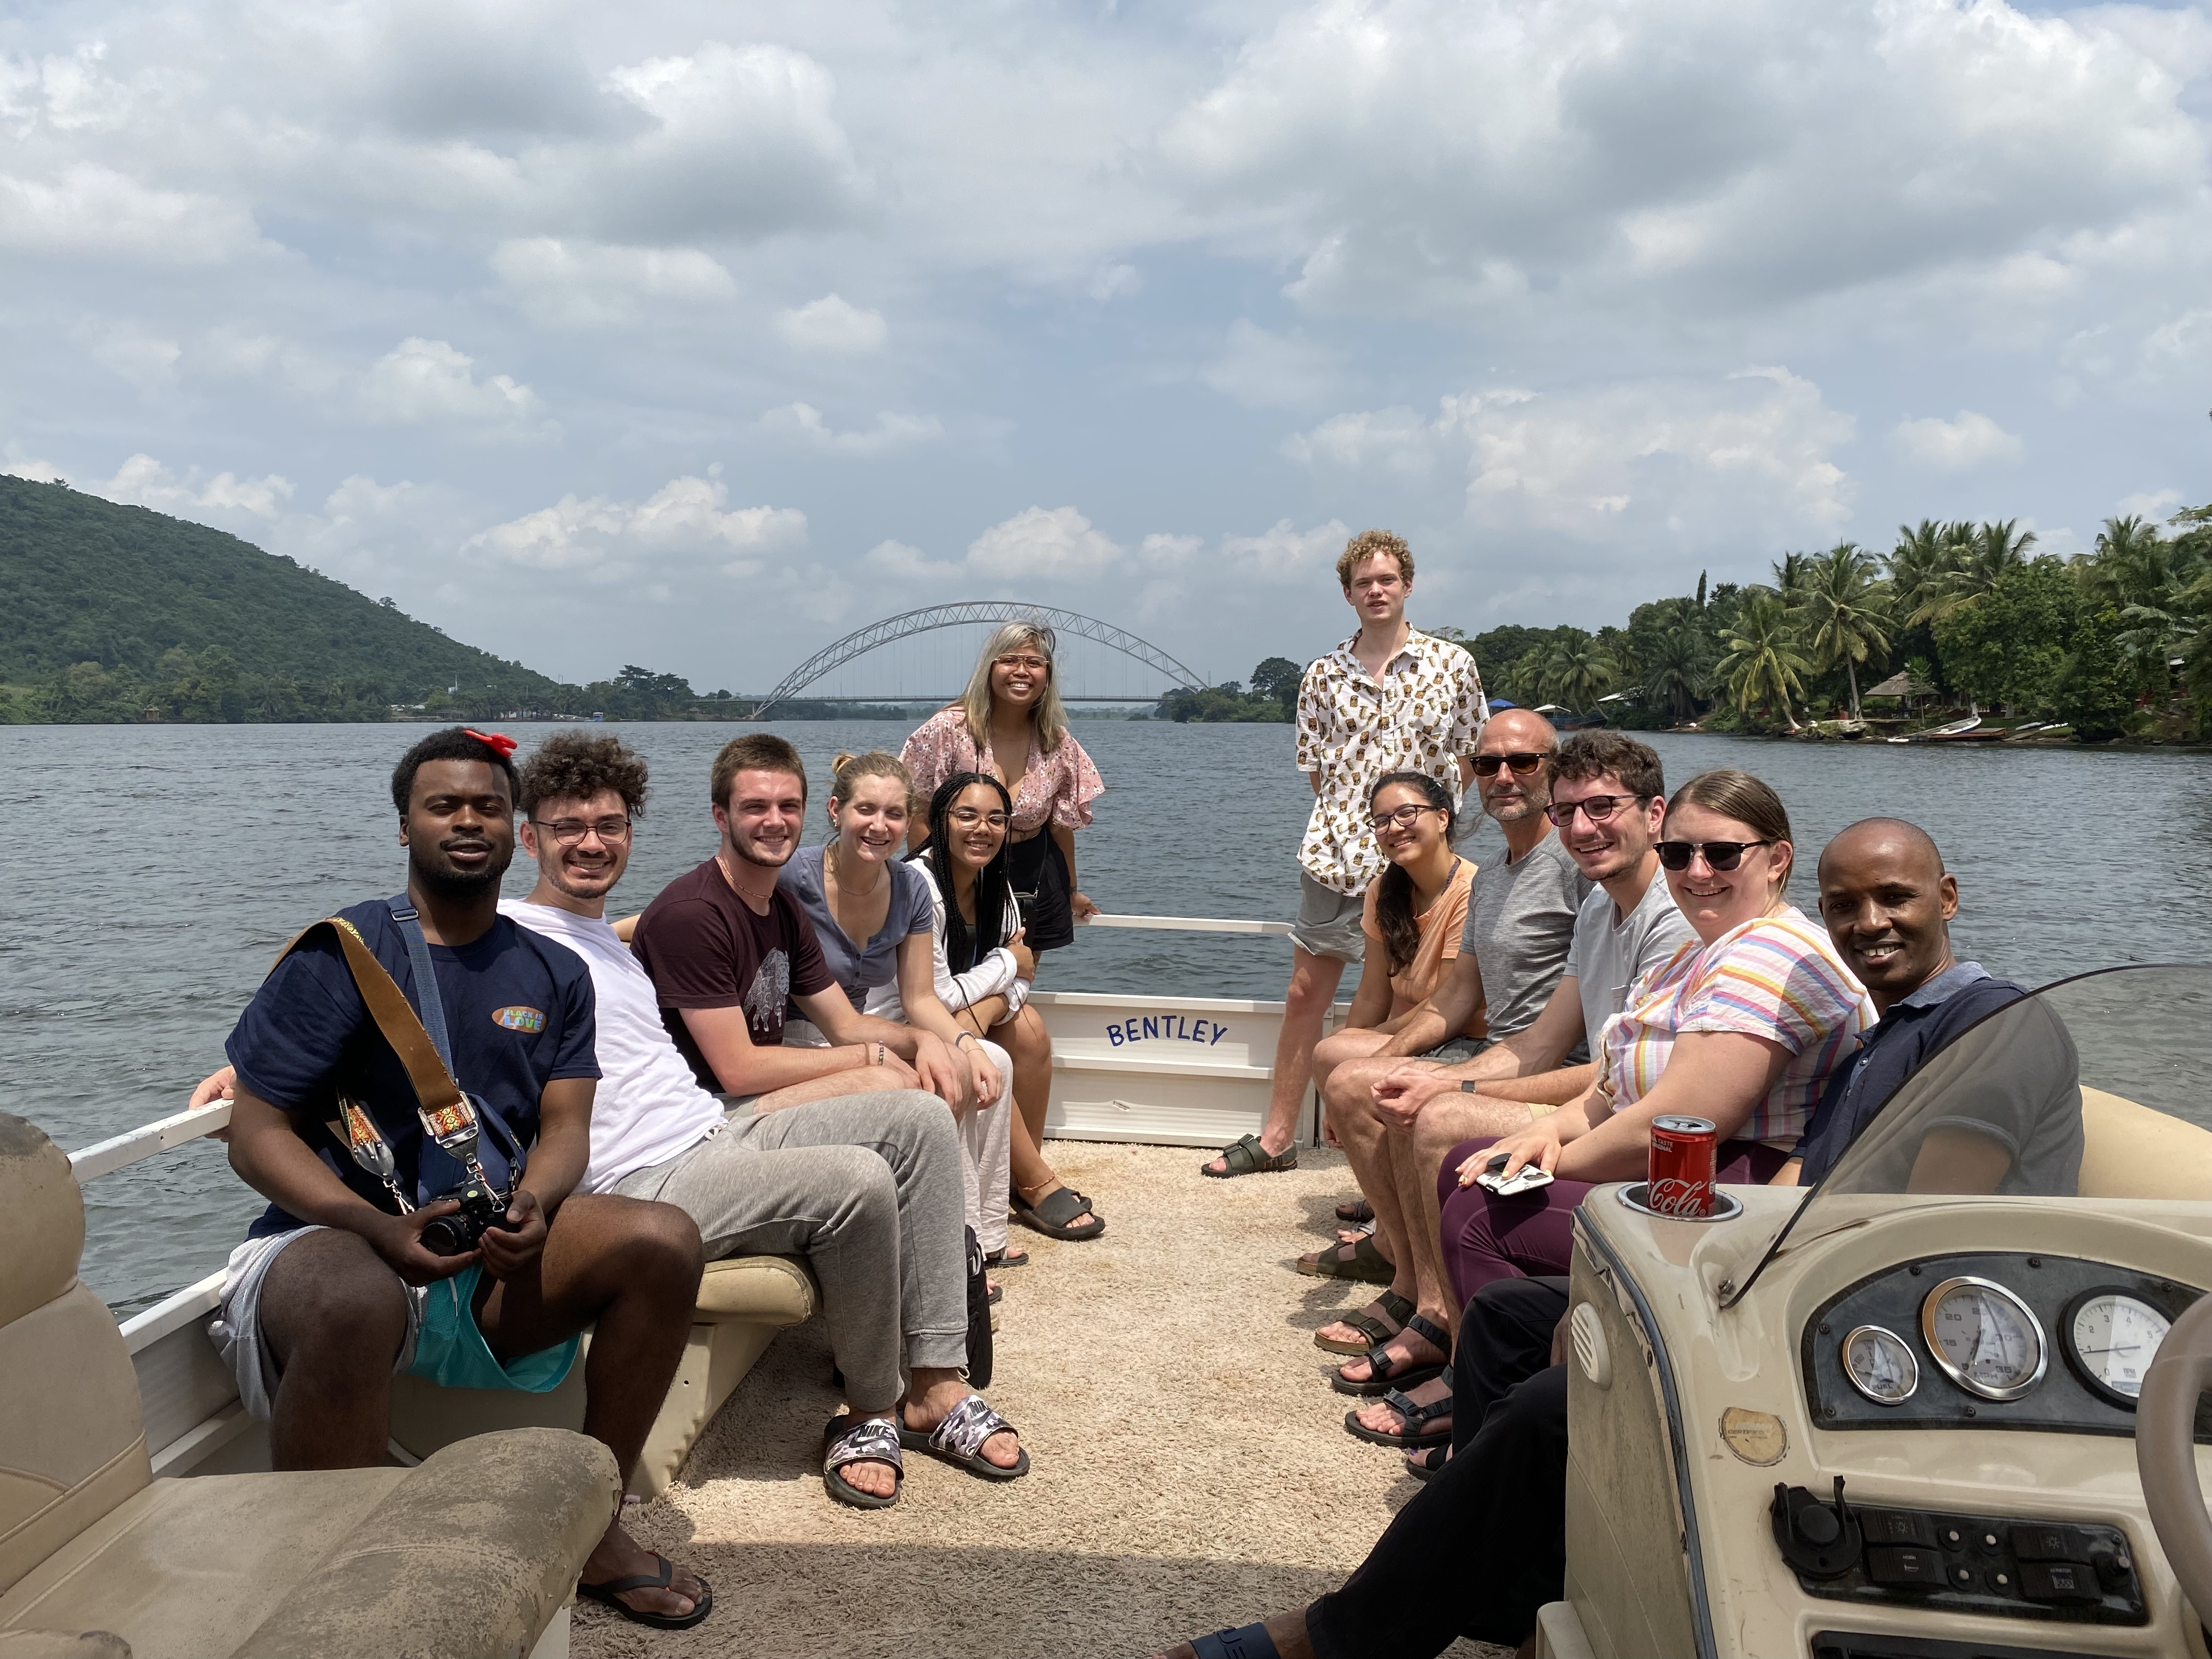
\includegraphics{IMG_0998.jpg}
\caption{Ghana}
\end{figure}

\begin{center}\rule{0.5\linewidth}{0.5pt}\end{center}

\hypertarget{study-objectives}{%
\section{STUDY OBJECTIVES}\label{study-objectives}}

\hypertarget{the-goal-is-to-provide-a-comprehensive-overview-of-this-trend-by-focusing-on-three-main-areas}{%
\subsection{The goal is to provide a comprehensive overview of this
trend by focusing on three main
areas:}\label{the-goal-is-to-provide-a-comprehensive-overview-of-this-trend-by-focusing-on-three-main-areas}}

\hypertarget{views-of-climate-change-among-millennials-and-generation-z}{%
\subsubsection{1. Views of climate change among Millennials and
Generation
Z}\label{views-of-climate-change-among-millennials-and-generation-z}}

\hypertarget{the-distribution-and-subsequent-interpretation-of-media-messages-on-climate-change}{%
\subsubsection{2. The distribution and subsequent interpretation of
media messages on climate
change}\label{the-distribution-and-subsequent-interpretation-of-media-messages-on-climate-change}}

\hypertarget{the-impact-these-perceptions-have-on-family-planning}{%
\subsubsection{3. The impact these perceptions have on family
planning}\label{the-impact-these-perceptions-have-on-family-planning}}

\begin{center}\rule{0.5\linewidth}{0.5pt}\end{center}

\hypertarget{last-term}{%
\section{LAST TERM}\label{last-term}}

\begin{figure}
\centering
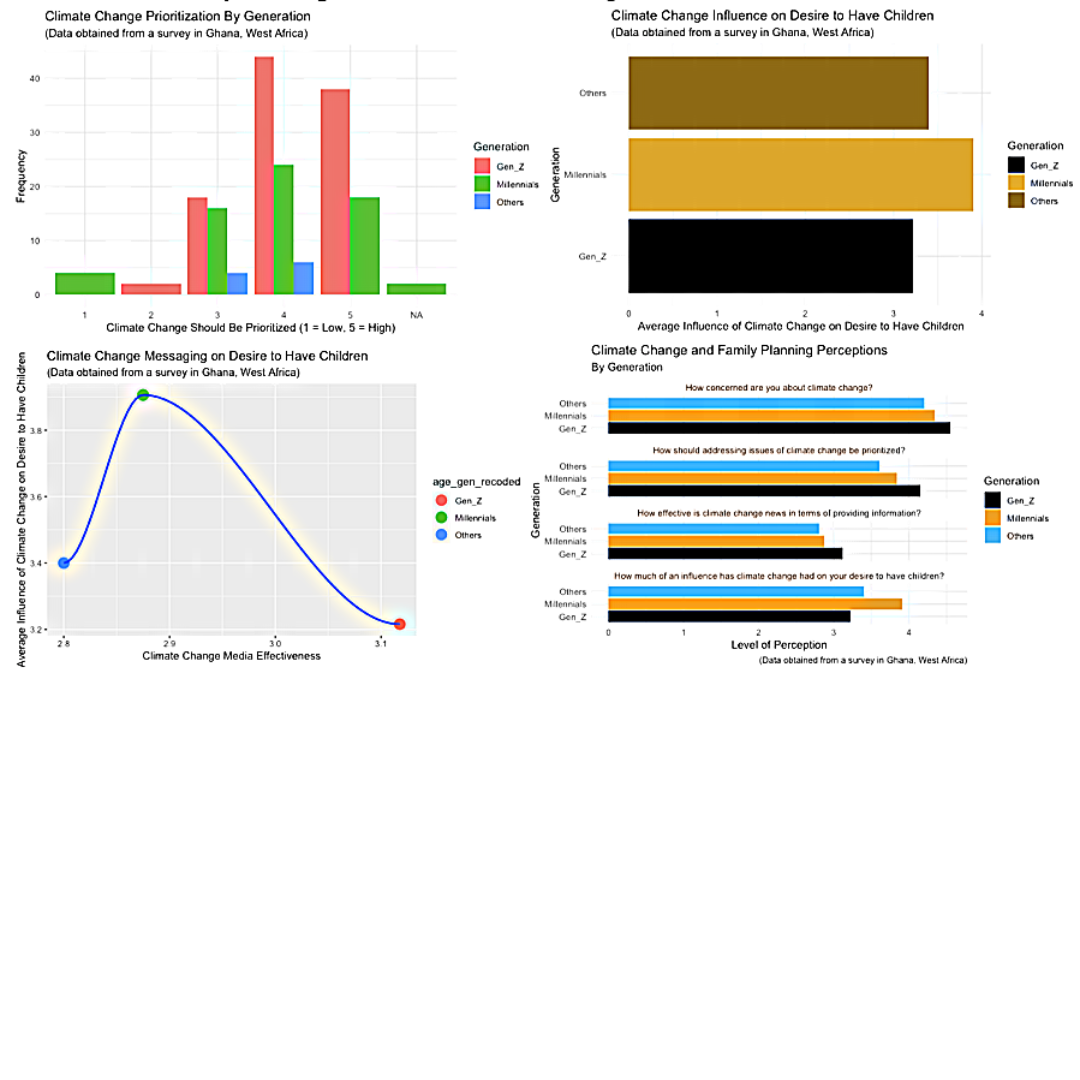
\includegraphics{v1.png}
\caption{New}
\end{figure}

\hypertarget{research-questions}{%
\section{RESEARCH QUESTIONS}\label{research-questions}}

\hypertarget{question-1-how-concerned-are-you-about-climate-change}{%
\subsubsection{Question 1: How concerned are you about climate
change?}\label{question-1-how-concerned-are-you-about-climate-change}}

\hypertarget{question-2-currently-how-much-is-the-issue-of-climate-change-being-addressed-in-the-region}{%
\subsubsection{Question 2: Currently, how much is the issue of climate
change being addressed in the
region}\label{question-2-currently-how-much-is-the-issue-of-climate-change-being-addressed-in-the-region}}

where you reside?

\hypertarget{question-3-how-much-of-an-influence-has-climate-change-had-on-your-desire-to-have-children}{%
\subsubsection{Question 3: How much of an influence has climate change
had on your desire to have
children?}\label{question-3-how-much-of-an-influence-has-climate-change-had-on-your-desire-to-have-children}}

\hypertarget{question-4-if-issues-of-climate-change-were-addressed-more-effectively-how-much-would-it-impact-your}{%
\subsubsection{Question 4: If issues of climate change were addressed
more effectively, how much would it impact
your}\label{question-4-if-issues-of-climate-change-were-addressed-more-effectively-how-much-would-it-impact-your}}

desire to have children?

\begin{center}\rule{0.5\linewidth}{0.5pt}\end{center}

\hypertarget{sample-visualization}{%
\section{SAMPLE VISUALIZATION}\label{sample-visualization}}

\begin{figure}
\centering
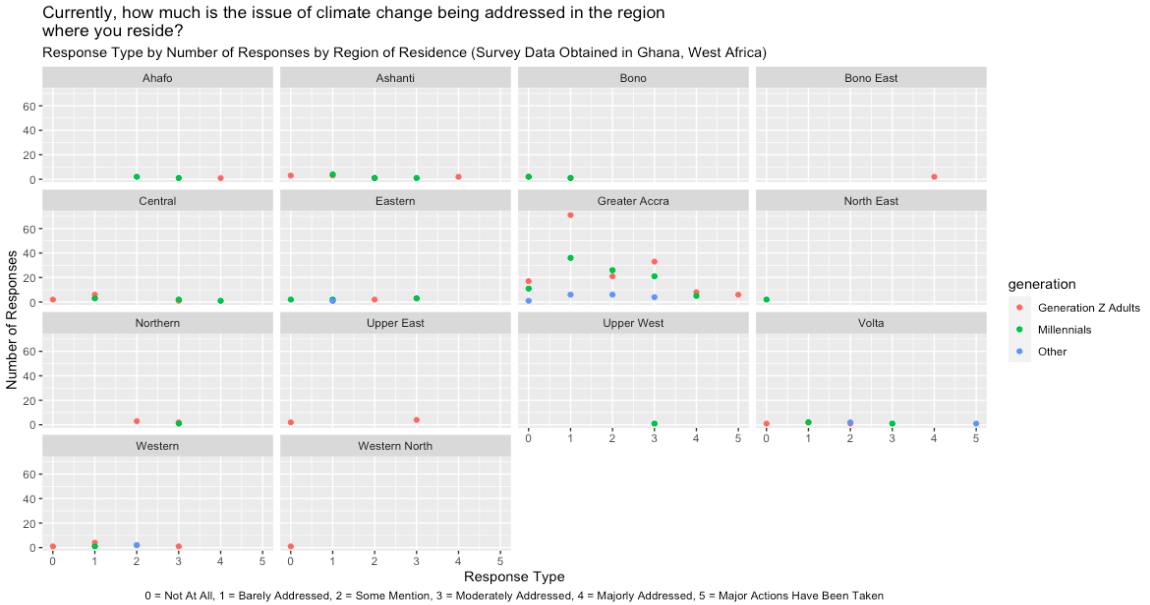
\includegraphics{Sample.png}
\caption{Sample}
\end{figure}

\begin{center}\rule{0.5\linewidth}{0.5pt}\end{center}

\hypertarget{thank-you}{%
\section{THANK YOU!}\label{thank-you}}

\begin{figure}
\centering
\includegraphics{https://images.emojiterra.com/google/android-nougat/512px/1f477-1f3fb-2640.png}
\caption{Thank You}
\end{figure}

\end{document}
